\documentclass[12pt]{article}

\usepackage{xeCJK}
\setCJKmainfont{FandolSong-Regular} % Ensure Fandol font is installed
\usepackage{titlesec}
\usepackage[utf8]{inputenc}
\usepackage{amsmath}
\usepackage{graphicx}
\usepackage{hyperref}
\usepackage{geometry}
\usepackage{fontspec}
\usepackage{float}


\geometry{a4paper, margin=1in}
\setmainfont{Times New Roman} % 设置主字体为 Times New Roman
%设置标题加粗 14号 times new roman

\title{\fontsize{14}{16}\bfseries 使用大语言模型的网页前端开发}
\author{\small Sanfeng Xin\\ \small by2410222@buaa.edu.cn}
\date{}

\begin{document}



\maketitle
\renewcommand{\abstractname}{\textbf{\Large Abstract}} % 修改摘要标题格式
\begin{abstract}
    近年来,大语言模型(LLMs)在自然语言处理领域取得了突破性进展,其强大的代码生成与理解能力使其在软件开发中展现出巨大潜力。本文探讨了大语言模型在网页前端开发中的应用方式,包括代码自动生成、组件设计、调试辅助等方面。我们以具体实践为例,评估了对比了 ChatGPT-4o\cite{openai2024gpt4ocard}与Qwen3\cite{yang2025qwen3technicalreport}模型在前端开发流程中的实际效果,并分析其优势与局限性。实验表明,LLMs 能显著提升开发效率,降低入门门槛,但在可控性、上下文理解和项目维护方面仍需谨慎对待。
\end{abstract}

\section*{\centering Introduction}
网页前端开发作为软件工程的重要组成部分,涉及 HTML、CSS、JavaScript 及各类框架(如 React、Vue)的综合应用。传统前端开发依赖开发者手动编码与调试,工作量大、重复性强。随着大语言模型(如 GPT-4)的发展,其对自然语言与代码的深度理解能力为前端开发提供了全新范式:开发者通过自然语言描述需求,模型便可输出相应代码、解释行为甚至进行错误分析。本文尝试使用ChatGPT-4o与Qwen3模型,进行网页前端的开发,对比两者在实际开发中的表现。并分析大语言模型在前端开发中的优势与局限性。
\section*{\centering Methodology}

\subsection*{\centering 目标网页和提示词}
我们设计了一个简单的游戏官网,主要用于展示游戏的美术风格、玩法介绍以及突出游戏特点。根据这个任务,我们制定了以下提示词:
\begin{quote}
    制作一个游戏介绍网页,这是一款像素风的包含了Roughlike要素,在多种群系冒险、邂逅各种各样的伙伴,打造和升级自己的装备,和伙伴和宠物一起冒险的游戏。网页包括核心玩法的介绍,几个可能遇到的角色的介绍,一些装备和宠物的介绍。
\end{quote}

\subsection*{\centering 模型选择}
因为在网页设计上需要一定的美术资源,因而选用了具有较好多模态能力的GPT-4o模型和Qwen3模型。两者都支持自然语言输入,并能生成相应的HTML、CSS和JavaScript代码。同时具有生成图像的能力。

在这里我们选用简单的HTML网页,并没有使用复杂的前端框架(如React或Vue),也没使用JavaScript的复杂逻辑,只探究其前端设计能力。

在图片生成上,分别有头图、背景图的网页外观设计,还有角色、装备、宠物系统的内在设计。


\section*{\centering Conclusions}
GPT-4o与Qwen3模型生成的网页分别如下所示:
\begin{figure}[H]
    \centering
    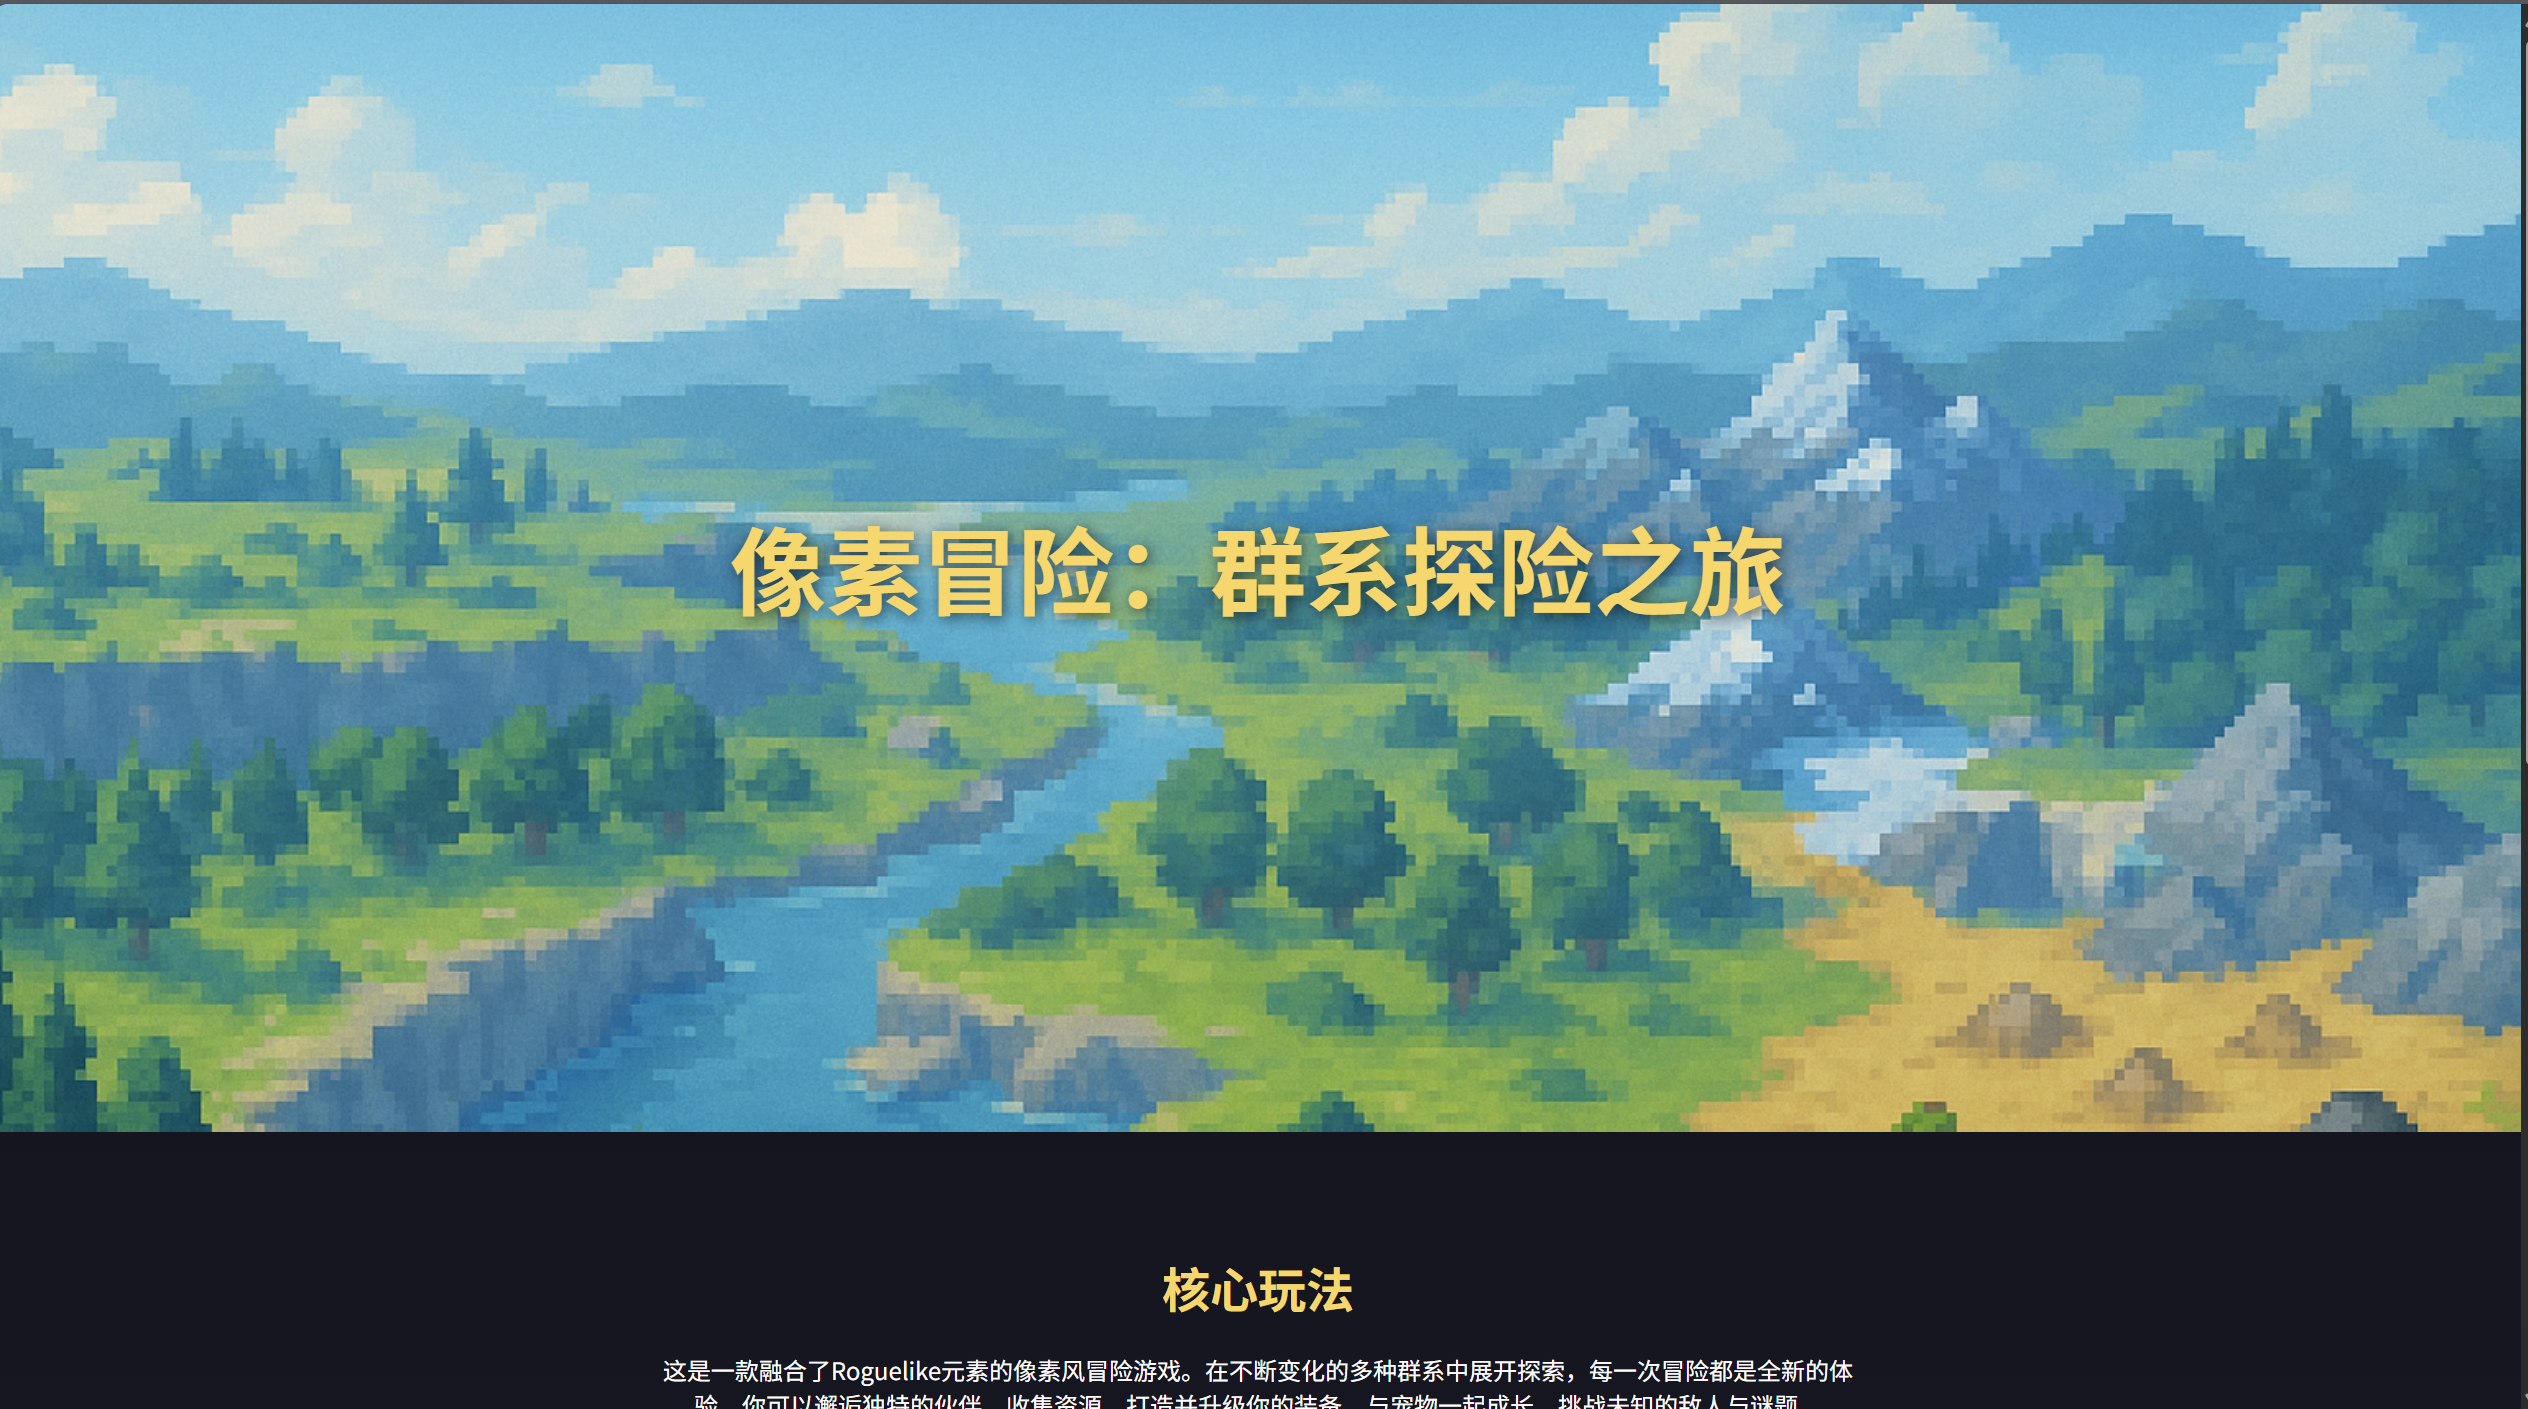
\includegraphics[width=0.8\textwidth]{gpt4o.png}
    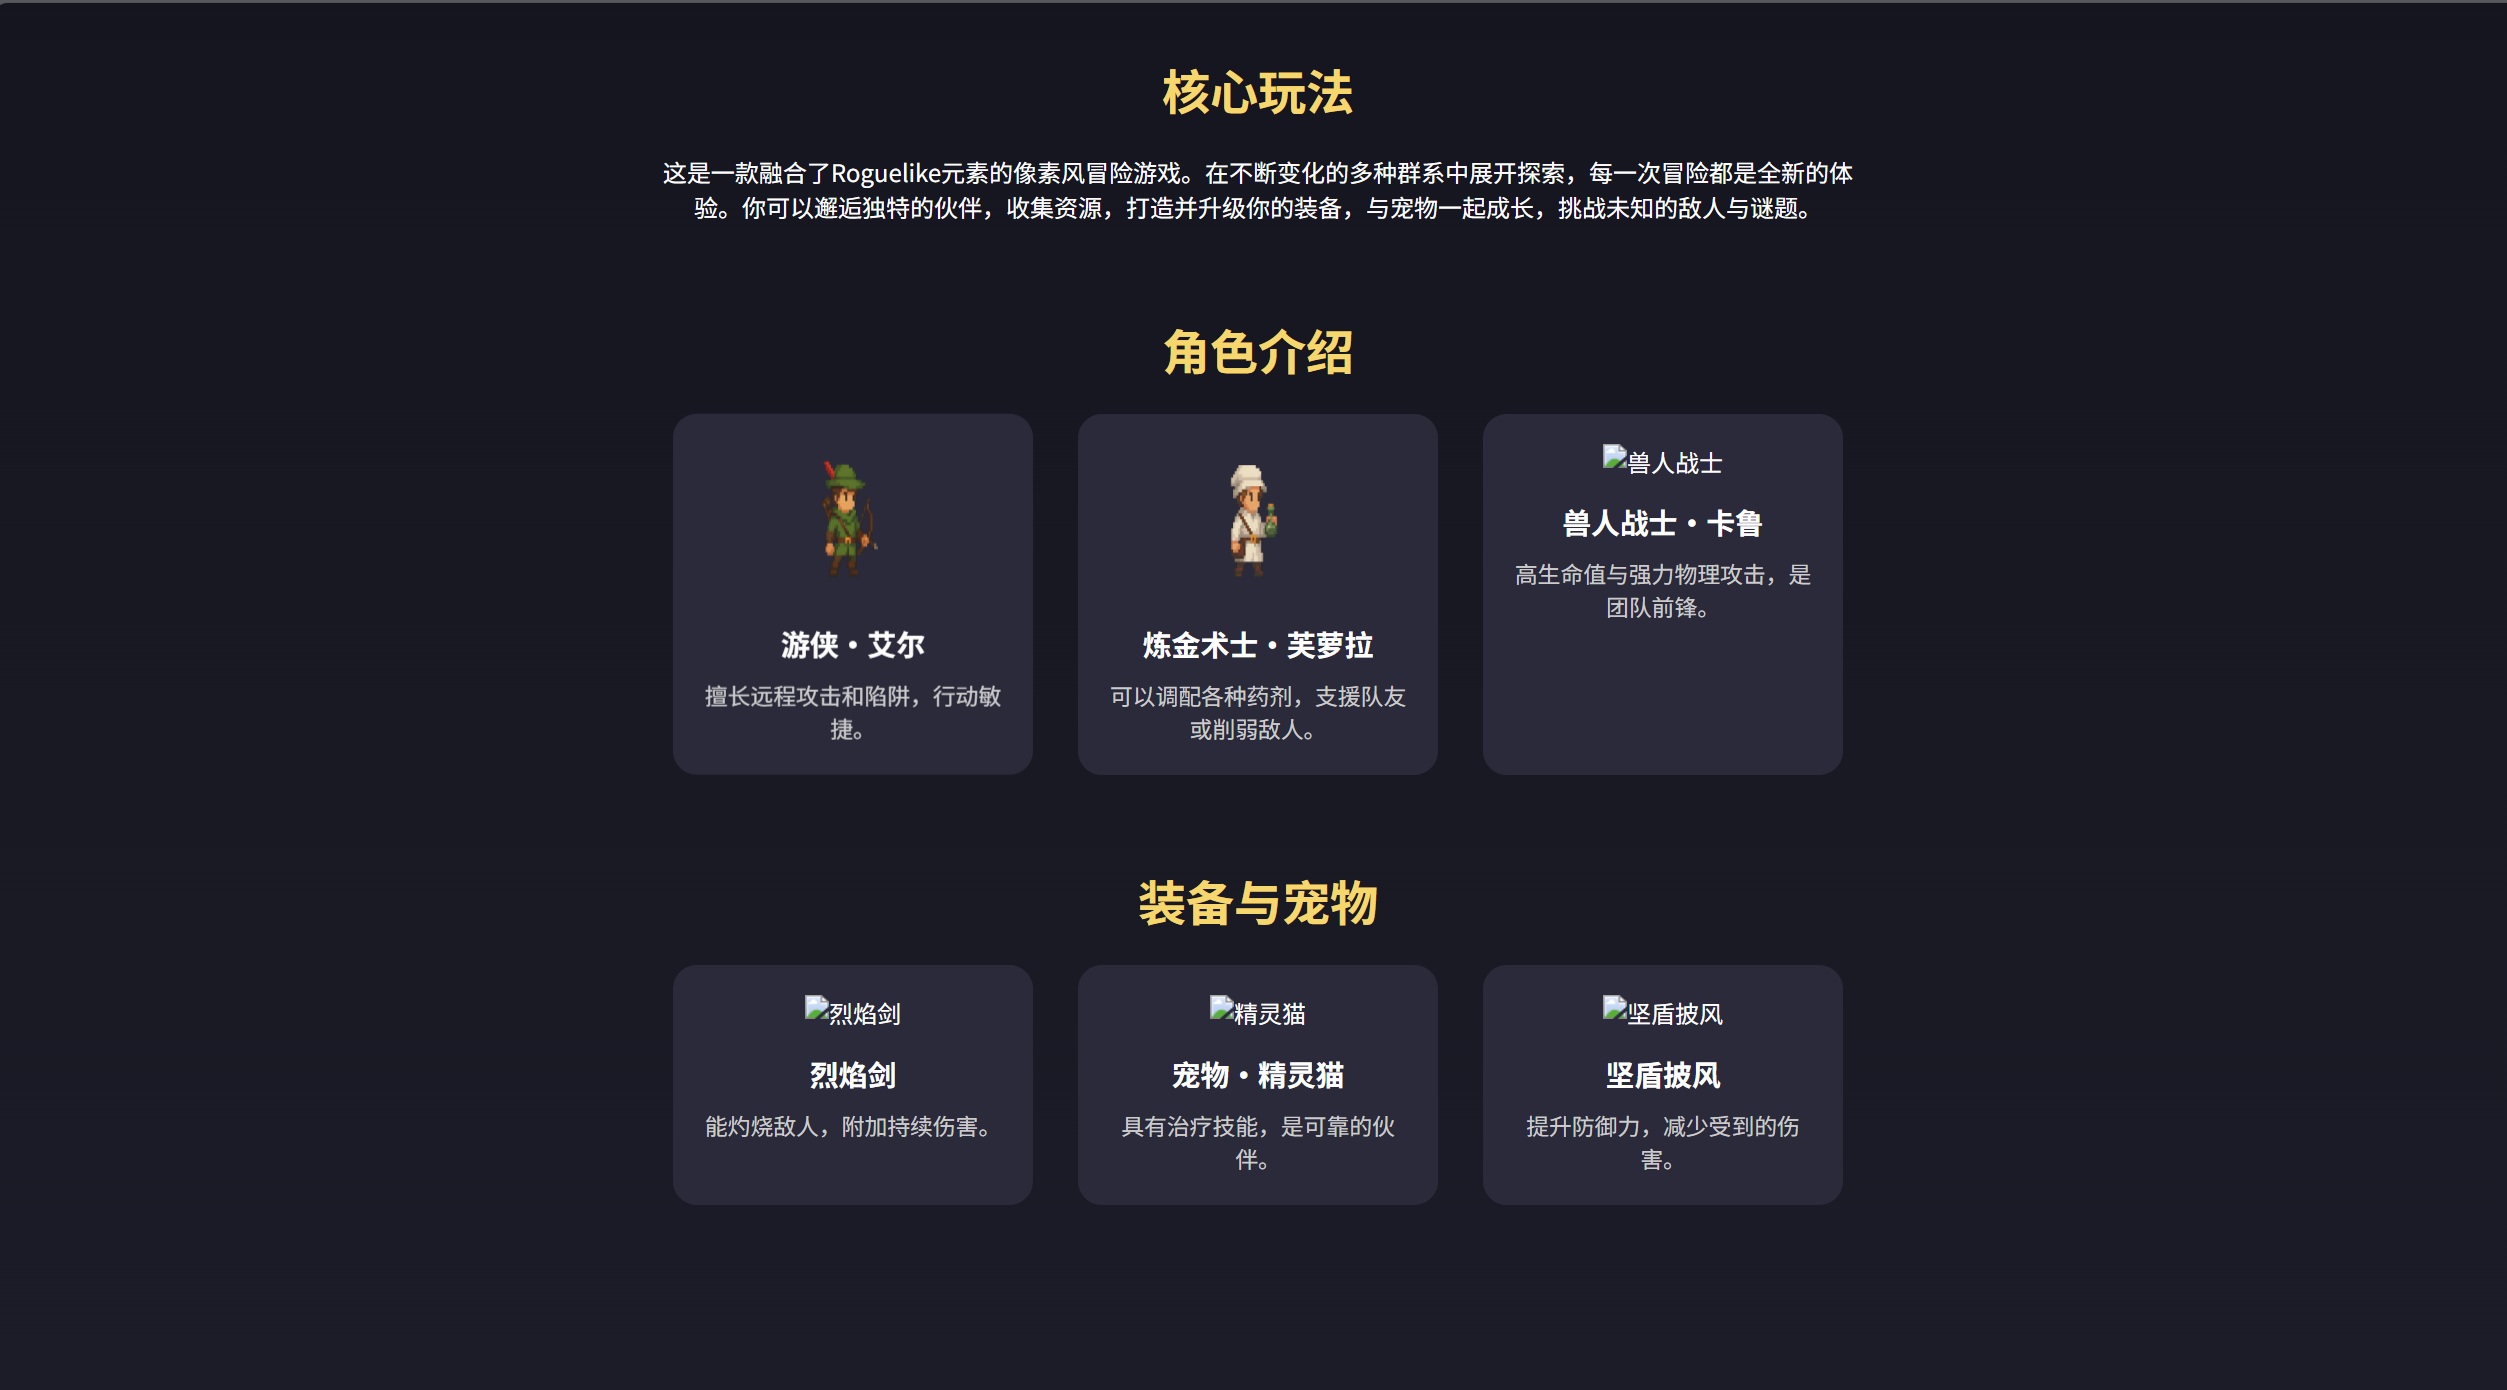
\includegraphics[width=0.8\textwidth]{gpt4o-2.png}
    \caption{GPT-4o生成的网页}
    \label{fig:gpt4o}
\end{figure}
\begin{figure}[H]
    \centering
    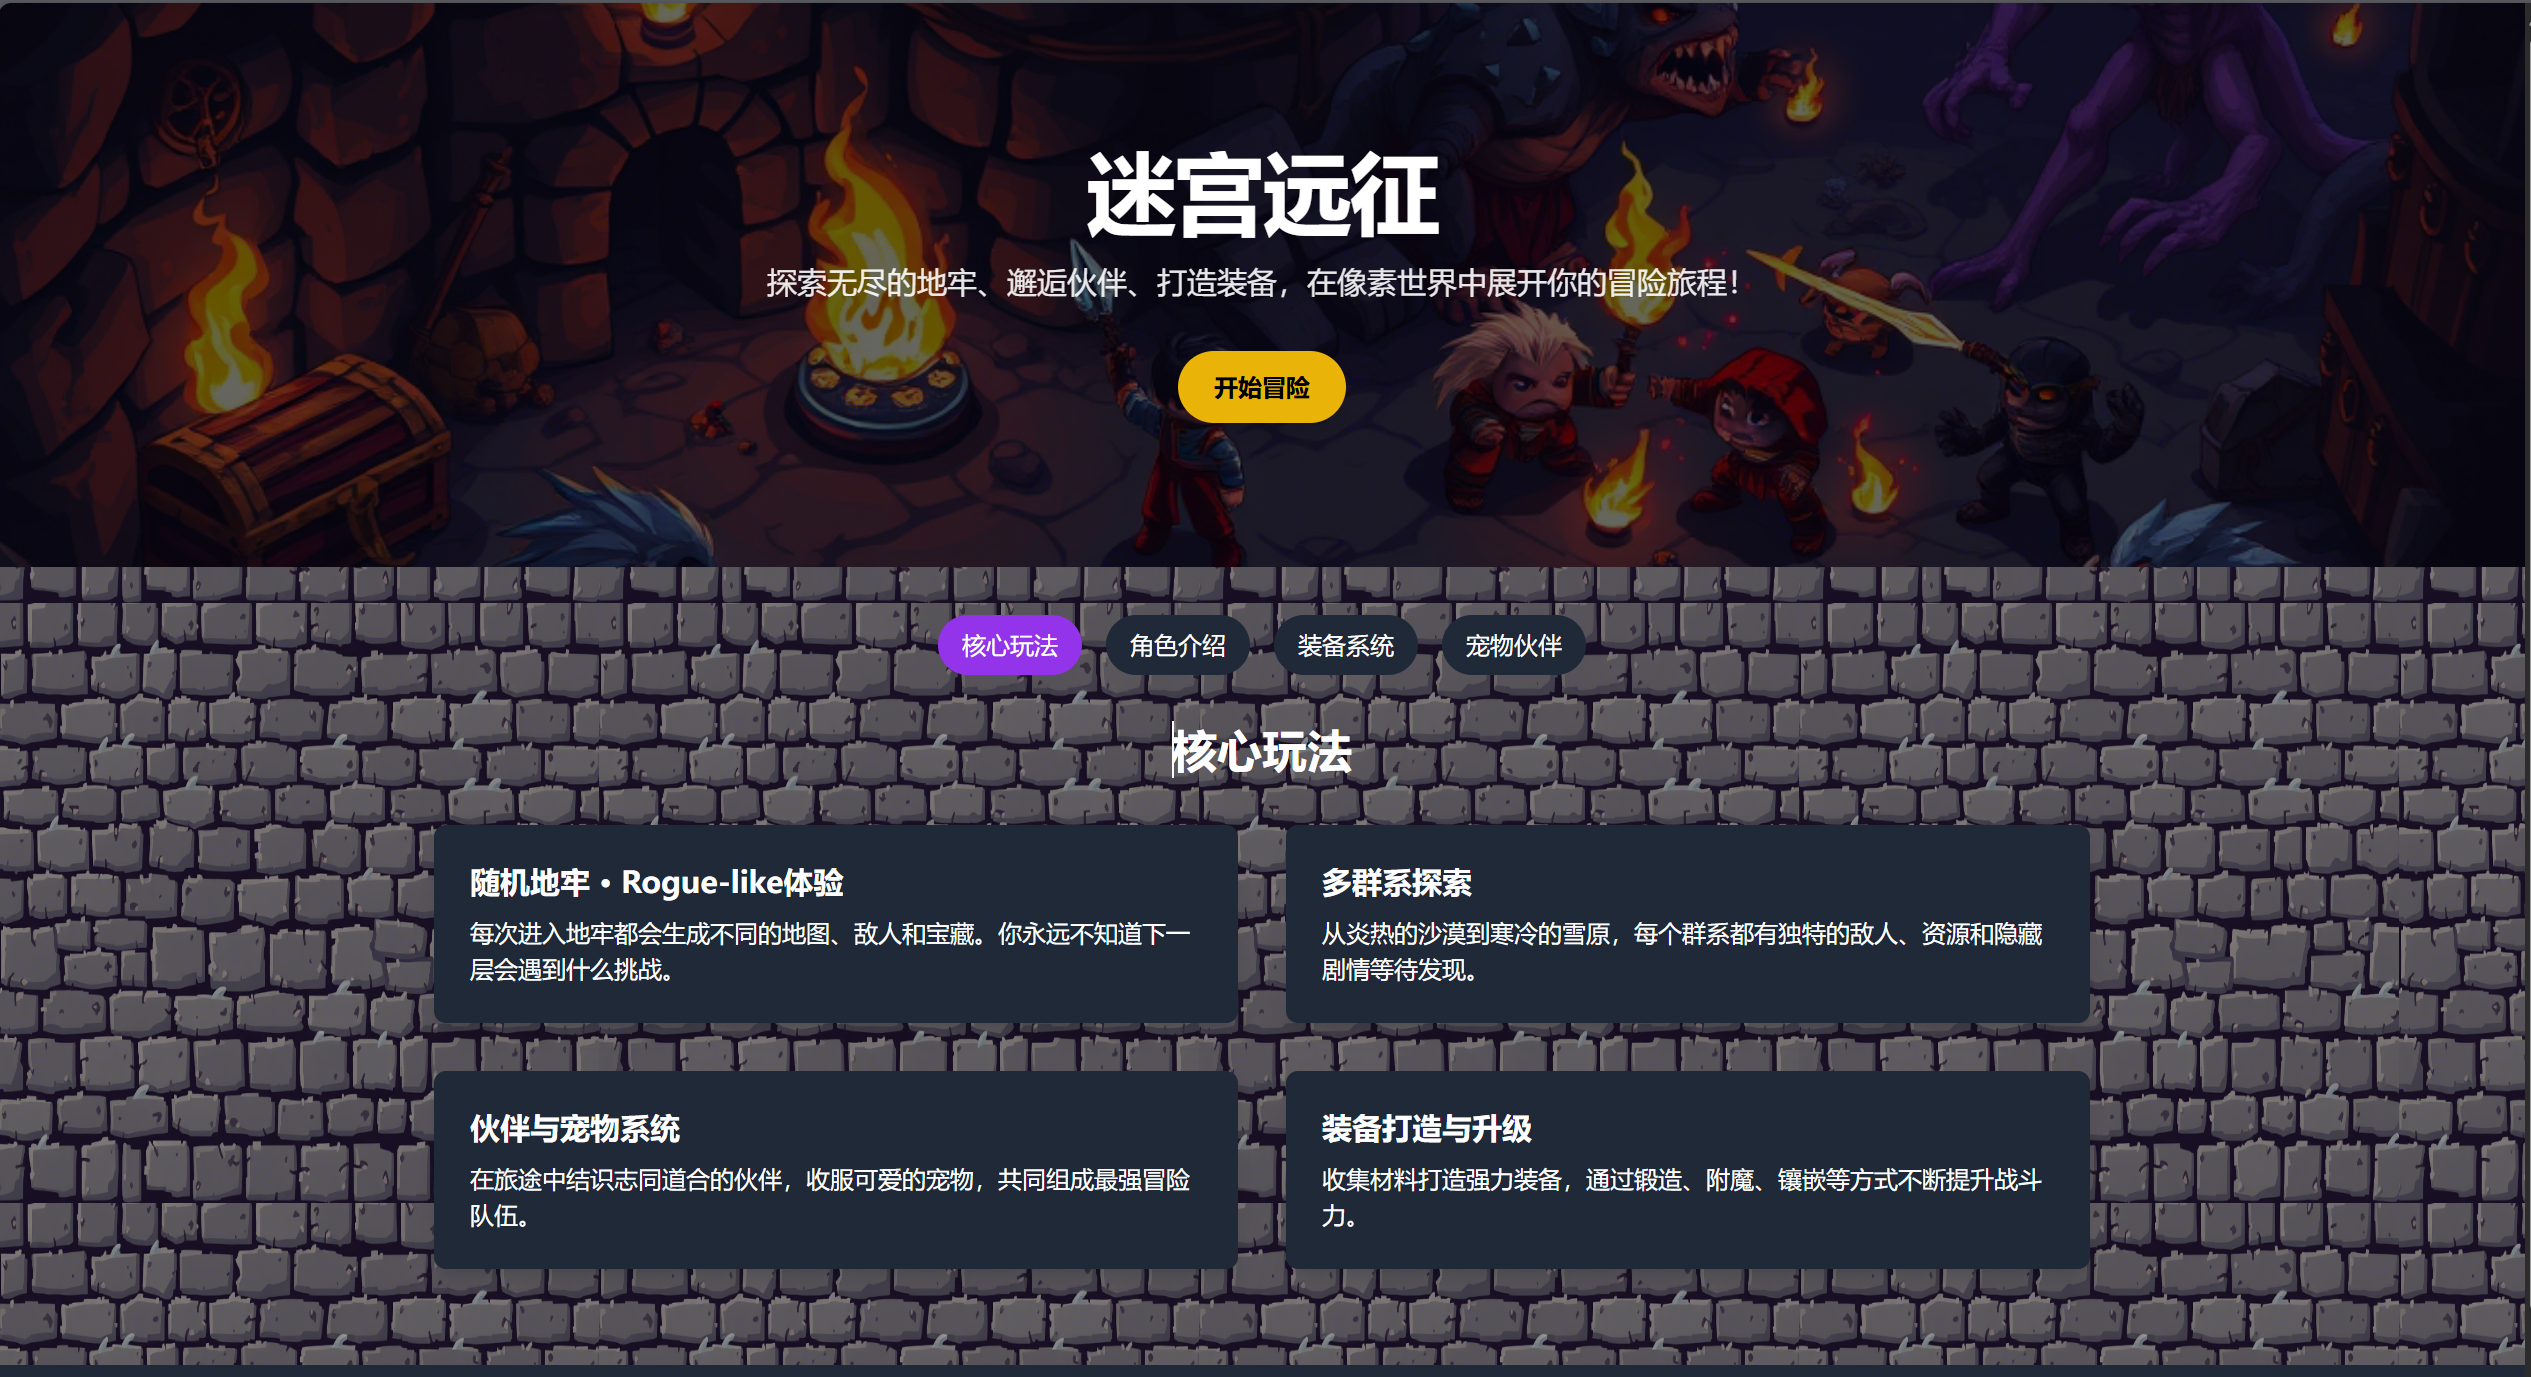
\includegraphics[width=0.8\textwidth]{qwen3.png}
    \caption{Qwen3生成的网页}
    \label{fig:qwen3}
\end{figure}
从网页设计上来看,GPT-4o生成的网页整体布局比较简单,但是比较大气,头图占到了比较大的面积,需要用户下划才能看到更加详细的内容。而Qwen3生成的网页则选择了以选项卡的形式呈现,将整体内容分为了四个选项卡:核心玩法、角色介绍、装备系统和宠物伙伴,更加直观清晰,同时还在底部添加了创作者的署名,比较完善。

在提示词较为简单模糊的情况下,Qwen3表现出更加出色的设计能力,能自己填充、设计内容的布局,风格上更为奔放。而GPT-4o表现的比较拘谨,但这也体现了其具有更好的可控性,在具有更详细提示词的情况下可能能给出更好的方案。
\begin{figure}[H]
    \centering
    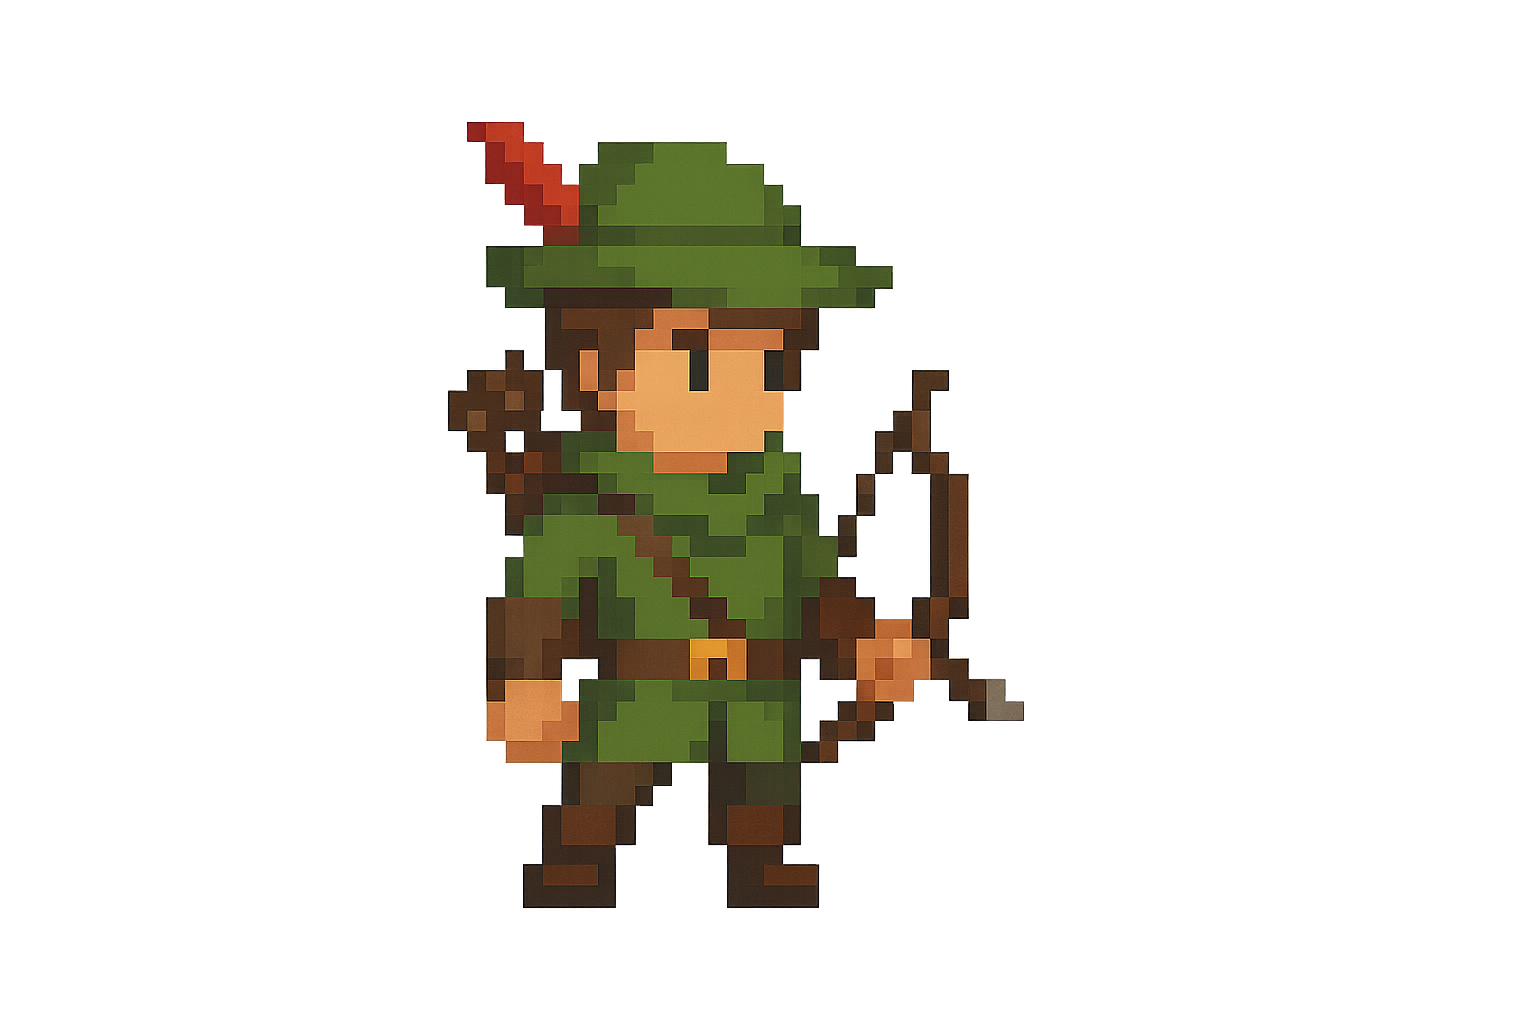
\includegraphics[width=0.8\textwidth]{youxia.png}
    
\includegraphics[width=0.8\textwidth]{lianjin.png}
    \caption{GPT-4o生成的角色图}
    \label{fig:gpt4o-image}
\end{figure}
\begin{figure}[H]
    \centering
    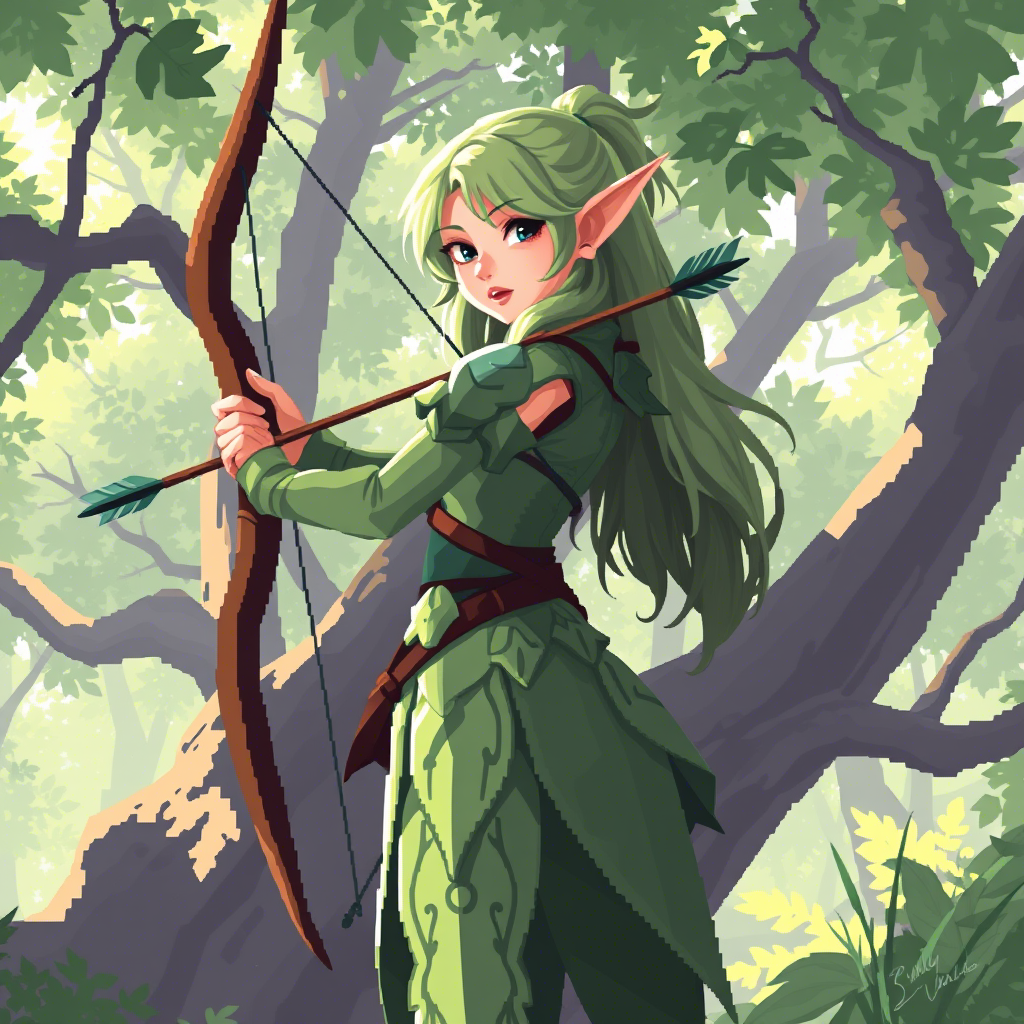
\includegraphics[width=0.8\textwidth]{images/elf.png}
    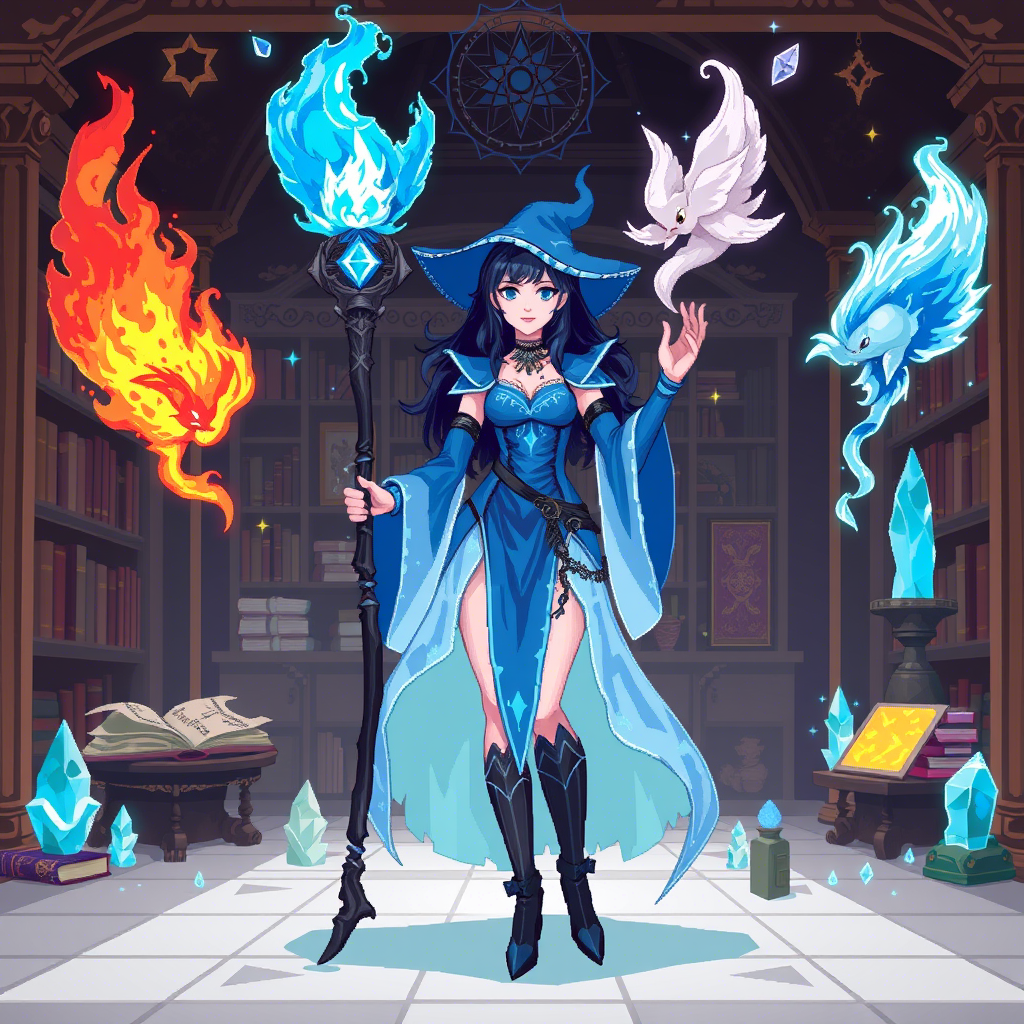
\includegraphics[width=0.8\textwidth]{images/caster.png}
    \caption{Qwen3生成的角色图}
    \label{fig:qwen3-image}
\end{figure}
在美术资源的生成上,二者的风格有所差异,但GPT-4o在对提示词、上下文的理解中表现更好,生成的图片更符合我的预想,同时在不同美术资源间的风格一致性也保持的更好。Qwen3在图像生成中体现了较差的记忆能力,生成的图片风格差异较大,不能直接在项目中使用。这可能也与提示词较为简单模糊有关,但在处理较长的提示词,更多的要求时,其只能满足部分要求,同时不能根据一张已有的图片来制作一张风格类似的图片。

总的来说,GPT-4o与Qwen3在网页前端开发中各有优势。GPT-4o在代码生成、上下文理解和图像生成方面表现更为出色,适合需要高可控性和一致性的项目。而Qwen3则在设计布局和创意表达上更为奔放,适合快速原型设计和创意探索。两者的结合可以为前端开发提供更全面的支持。大语言模型在网页前端开发中展现出强大的潜力,但仍需注意其局限性,如可控性、上下文理解和项目维护等问题。未来,随着模型的不断优化与发展,我们有理由相信大语言模型将在前端开发领域发挥更大的作用。
\section*{\centering References}


\bibliographystyle{plain}
\bibliography{reference}


\end{document}